A demo showing an example of Event Based PSHA calculation is provided with the
following configuration file:

\begin{Verbatim}[frame=single, commandchars=\\\{\}, fontsize=\normalsize]
[general]
description = Event Based PSHA using Area Source
calculation_mode = event_based
random_seed = 23

[geometry]
sites = 0.5 -0.5

[logic_tree]
number_of_logic_tree_samples = 0

[erf]
rupture_mesh_spacing = 2
width_of_mfd_bin = 0.1
area_source_discretization = 5.0

[site_params]
reference_vs30_type = measured
reference_vs30_value = 600.0
reference_depth_to_2pt5km_per_sec = 5.0
reference_depth_to_1pt0km_per_sec = 100.0

[calculation]
source_model_logic_tree_file = source_model_logic_tree.xml
gsim_logic_tree_file = gmpe_logic_tree.xml
investigation_time = 50.0
intensity_measure_types_and_levels = {"PGA": [...]}
truncation_level = 3
maximum_distance = 200.0

[event_based_params]
ses_per_logic_tree_path = 100
ground_motion_correlation_model =
ground_motion_correlation_params =

[output]
export_dir = ...
ground_motion_fields = true
hazard_curves_from_gmfs = true
mean = false
quantiles = 
hazard_maps = true
poes = 0.1
\end{Verbatim}

The source model consist of one source (area). 100 stochastic event sets  are
generated (\texttt{ses\_\-per\_\-logic\_\-tree\_\-path = 100}) (an example
can be seen in Figure~\ref{fig:ses}). Ground motion fields are computed
(\texttt{ground\_\-motion\_\-fields = true}, Figure~\ref{fig:gmfs}) and also
hazard curves from ground motion fields are extracted
(\texttt{hazard\_\-curves\_\-from\_\-gmfs = true}). The corresponding hazard
maps for 0.1 probability are also calculated (\texttt{hazard\_\-maps = true})

\begin{figure}
\centering
\subcaptionbox{}
{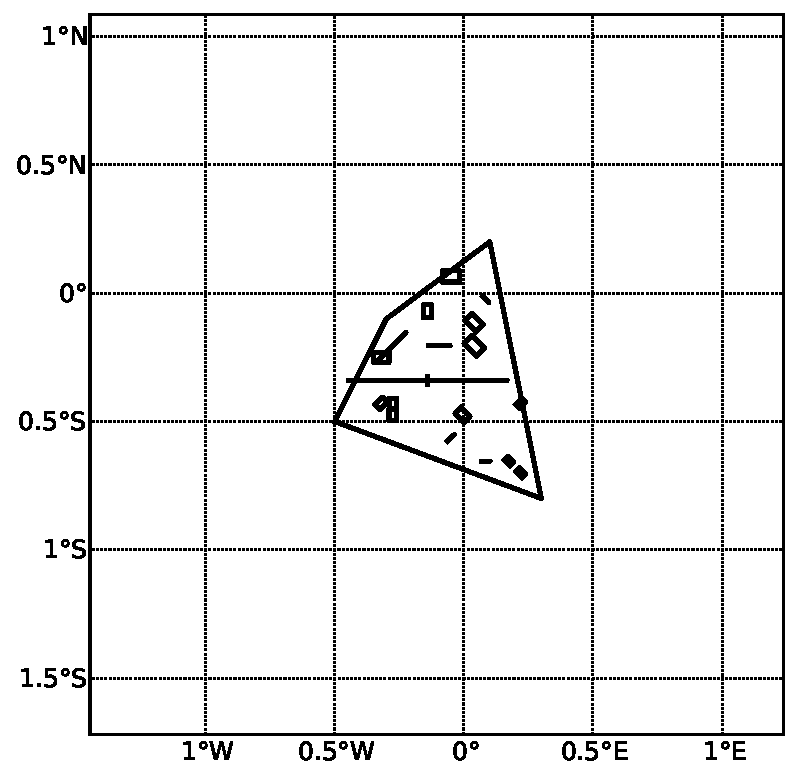
\includegraphics[width=9cm]{figures/hazard/ses.pdf}} 
\caption{A stochastic event set generated with the event based PSHA demo. 
    The area source defines a nodal plane distribution which distributes 
    events among vertical and dipping (50 degrees) faults with equal weights. 
    Vertical ruptures are then distributed equally in the range 0-180 degrees 
    while the dipping ones in the range 0-360, both with a step of 45 degrees.}
\label{fig:ses}
\end{figure}

\begin{figure}
\centering
\subcaptionbox{}
{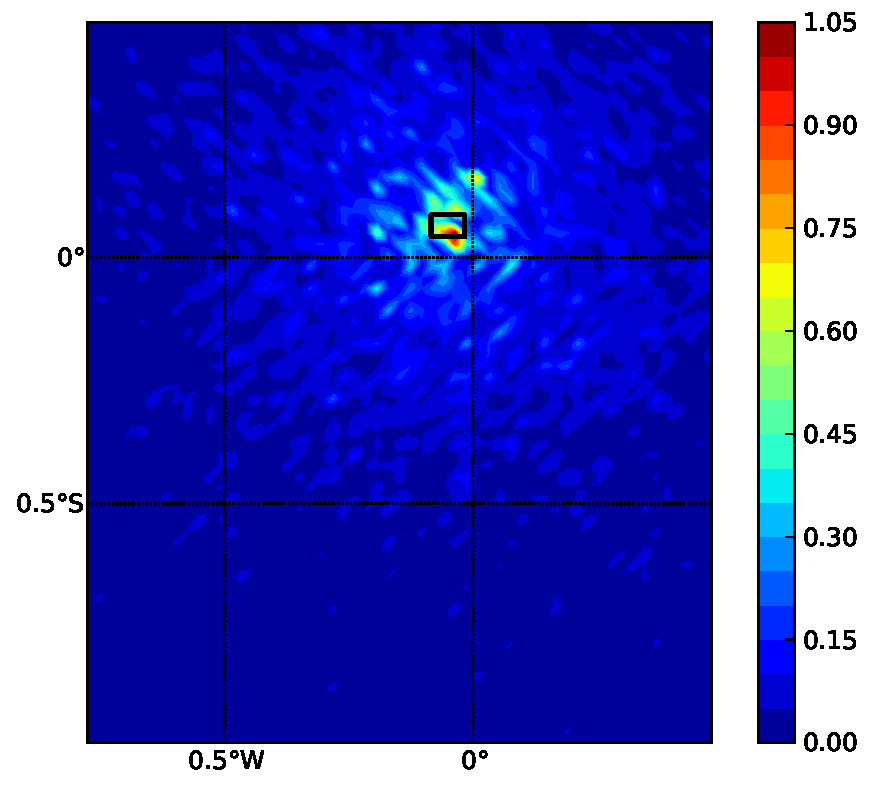
\includegraphics[width=6cm]{figures/hazard/gmf-no-corr.pdf}} 
\subcaptionbox{}
{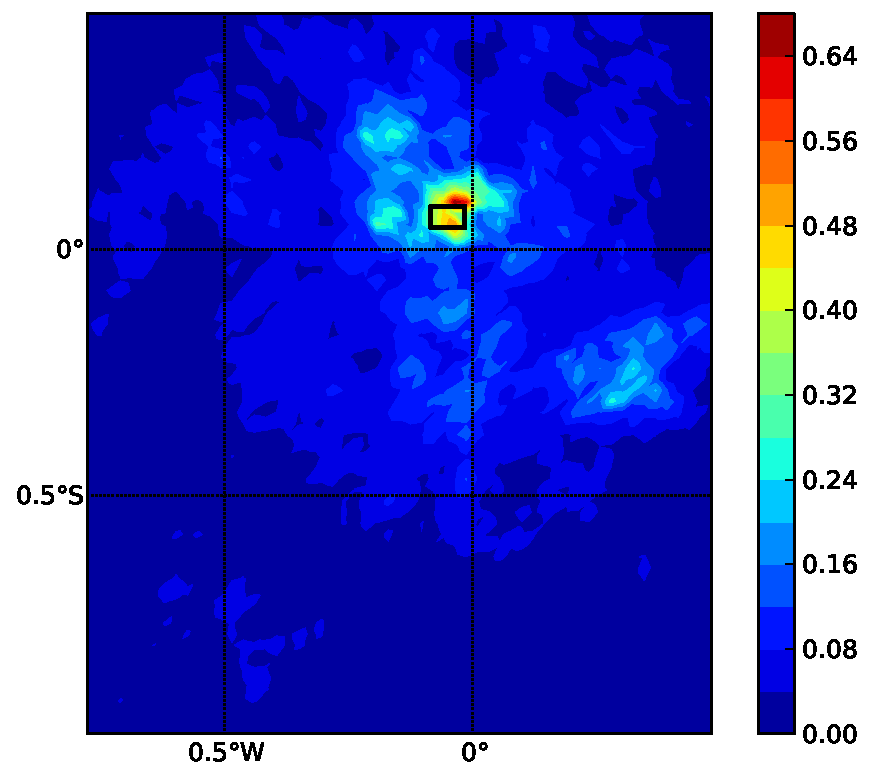
\includegraphics[width=6cm]{figures/hazard/gmf-corr.pdf}} 
\caption{Ground motion fields (PGA) with no spatial correlations (a) and with spatial correlation (b)}
\label{fig:gmfs}
\end{figure}